\documentclass{standalone}
\usepackage[dvipsnames]{xcolor}
\usepackage{tikz}
\newcommand{\drawMineUnvisited}[1]{\draw [lightgray, fill=lightgray, fill opacity=0.5] #1 circle [radius=0.4]}
\newcommand{\drawMineFrontier}[1]{\draw [SkyBlue, fill=SkyBlue, fill opacity=0.5] #1 circle [radius=0.4]}
\newcommand{\drawMineVisited}[1]{\draw [orange, fill=orange, fill opacity=0.5] #1 circle [radius=0.4]}
\newcommand{\drawMineFound}[1]{\draw [green, fill=green, fill opacity=0.5] #1 circle [radius=0.4]}
\newcommand{\drawMineNotFound}[1]{\draw [black, fill=black, fill opacity=0.9] #1 circle [radius=0.4]}


\begin{document}
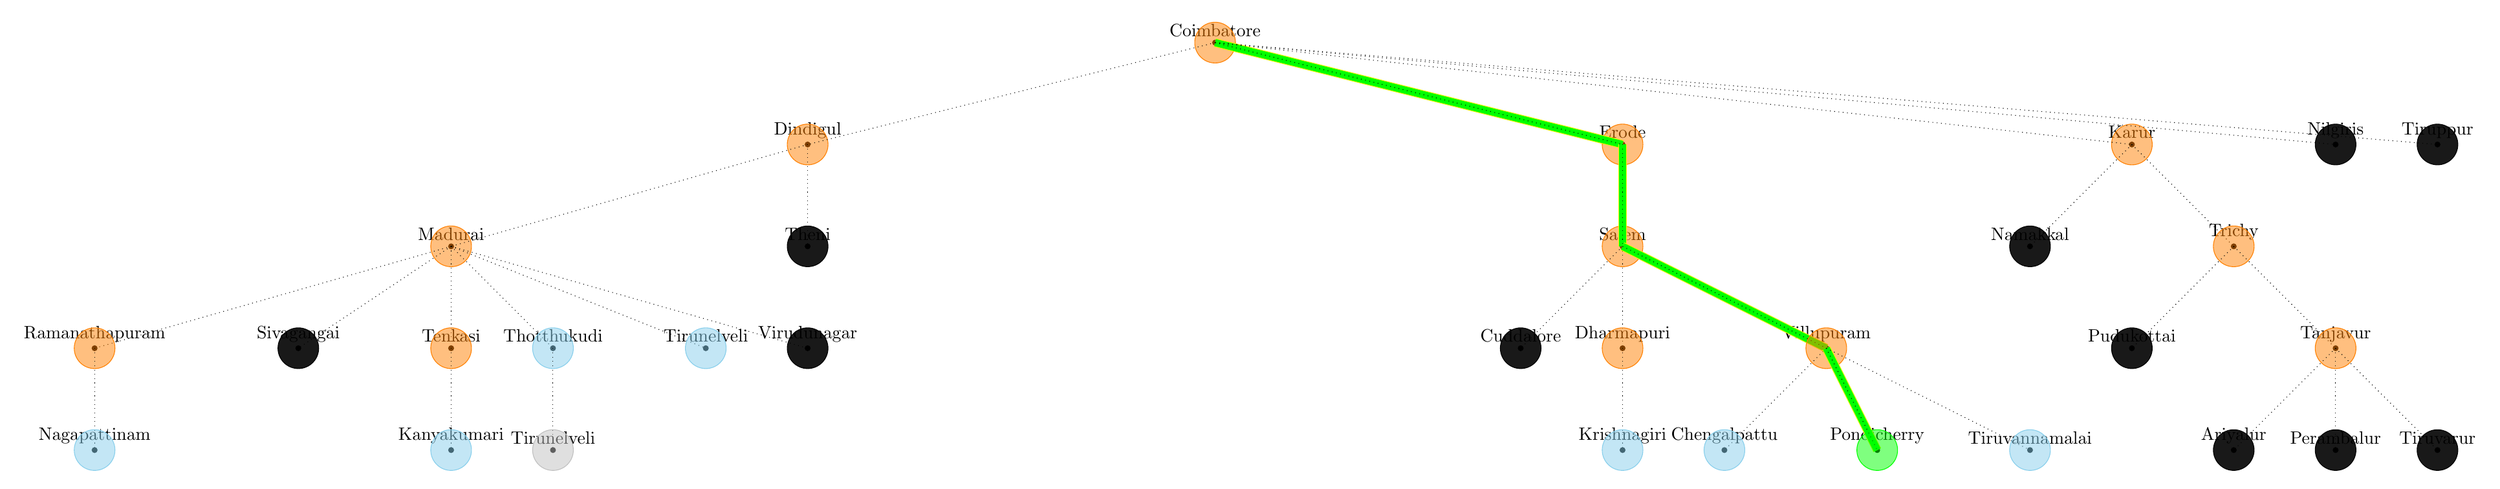
\begin{tikzpicture}
    \draw [black, fill=black ] (-18,0) circle [radius=0.05] node[above] {Coimbatore};
    \drawMineVisited{(-18,0)};

    %for coimbatore
    \draw [fill=black] (-26,-2) circle [radius=0.05] node[above] {Dindigul};
    \drawMineVisited{(-26,-2)};
    \draw [ dotted] (-18,0) -- (-26,-2);

    \draw [fill=black] (-10,-2) circle [radius=0.05] node[above] {Erode};
    \drawMineVisited{(-10,-2)};
    \draw [ dotted, preaction={%But before that
    draw,yellow,-,% Draw yellow without any arrow head
    double=green,
    double distance=10\pgflinewidth,
    }] (-18,0) -- (-10,-2);

    \draw [fill=black] (0,-2) circle [radius=0.05] node[above] {Karur};
	\drawMineVisited{(-0,-2)};
    \draw [ dotted] (-18,0) -- (-0,-2);

    \draw [fill=black] (4,-2) circle [radius=0.05] node[above] {Nilgiris};
	\drawMineNotFound{(4,-2)};
    \draw [ dotted] (-18,0) -- (4,-2);

    \draw [fill=black] (6,-2) circle [radius=0.05] node[above] {Tiruppur};
	\drawMineNotFound{(6,-2)};
    \draw [ dotted] (-18,0) -- (6,-2);

    %for dindigul
    \draw [fill=black] (-33,-4) circle [radius=0.05] node[above] {Madurai};
	\drawMineVisited{(-33,-4)};
    \draw [ dotted] (-26,-2) -- (-33,-4);

    \draw [fill=black] (-26,-4) circle [radius=0.05] node[above] {Theni};
	\drawMineNotFound{(-26,-4)};
    \draw [ dotted] (-26,-2) -- (-26,-4);


    %for erode
    \draw [fill=black] (-10,-4) circle [radius=0.05] node[above] {Salem};
	\drawMineVisited{(-10,-4)};
    \draw [ dotted, preaction={%But before that
    draw,yellow,-,% Draw yellow without any arrow head
    double=green,
    double distance=10\pgflinewidth,
    }] (-10,-2) -- (-10,-4);

    %for karur
    \draw [fill=black] (-2,-4) circle [radius=0.05] node[above] {Namakkal};
    \draw [ dotted] (-0,-2) -- (-2,-4);
    \drawMineNotFound{(-2,-4)};

    \draw [fill=black] (2,-4) circle [radius=0.05] node[above] {Trichy};
    \draw [ dotted] (-0,-2) -- (2,-4);
    \drawMineVisited{(2,-4)};


    %for madurai
    \draw [fill=black] (-40,-6) circle [radius=0.05] node[above] {Ramanathapuram};
    \draw [ dotted] (-33,-4) -- (-40,-6);
    \drawMineVisited{(-40,-6)};

    \draw [fill=black] (-36,-6) circle [radius=0.05] node[above] {Sivagangai};
    \draw [ dotted] (-33,-4) -- (-36,-6);
    \drawMineNotFound{(-36,-6)};

    \draw [fill=black] (-33,-6) circle [radius=0.05] node[above] {Tenkasi};
    \draw [ dotted] (-33,-4) -- (-33,-6);
    \drawMineVisited{(-33,-6)};

    \draw [fill=black] (-31,-6) circle [radius=0.05] node[above] {Thotthukudi};
    \draw [ dotted] (-33,-4) -- (-31,-6);
    \drawMineFrontier{(-31,-6)};

    \draw [fill=black] (-28,-6) circle [radius=0.05] node[above] {Tirunelveli};
    \draw [ dotted] (-33,-4) -- (-28,-6);
    \drawMineFrontier{(-28,-6)};


    \draw [fill=black] (-26,-6) circle [radius=0.05] node[above] {Virudunagar};
    \draw [ dotted] (-33,-4) -- (-26,-6);
    \drawMineNotFound{(-26,-6)};
    %for Theni

    %for Trichy
    \draw [fill=black] (0,-6) circle [radius=0.05] node[above] {Pudukottai};
    \draw [ dotted] (2,-4) -- (-0,-6);
    \drawMineNotFound{(-0,-6)};

    \draw [fill=black] (4,-6) circle [radius=0.05] node[above] {Tanjavur};
    \draw [ dotted] (2,-4) -- (4,-6);
    \drawMineVisited{(4,-6)};

    %for Salem
    \draw [fill=black] (-12,-6) circle [radius=0.05] node[above] {Cuddalore};
    \draw [ dotted] (-10,-4) -- (-12,-6);
    \drawMineNotFound{(-12,-6)};

    \draw [fill=black] (-10,-6) circle [radius=0.05] node[above] {Dharmapuri};
    \draw [ dotted] (-10,-4) -- (-10,-6);
    \drawMineVisited{(-10,-6)};

    \draw [fill=black] (-6,-6) circle [radius=0.05] node[above] {Villupuram};
    \draw [ dotted, preaction={%But before that
    draw,yellow,-,% Draw yellow without any arrow head
    double=green,
    double distance=10\pgflinewidth,
    }] (-10,-4) -- (-6,-6);
    \drawMineVisited{(-6,-6)};

    %for Namakkal

    %for Ramanathapuram
    \draw [fill=black] (-40,-8) circle [radius=0.05] node[above] {Nagapattinam};
    \draw [ dotted] (-40,-6) -- (-40,-8);
    \drawMineFrontier{(-40,-8)};
    %for  Sivagangai

    %for Tenkasi
    \draw [fill=black] (-33,-8) circle [radius=0.05] node[above] {Kanyakumari};
    \draw [ dotted] (-33,-6) -- (-33,-8);
    \drawMineFrontier{(-33,-8)};

    %for Thoothukudi
    \draw [fill=black] (-31,-8) circle [radius=0.05] node[above] {Tirunelveli};
    \draw [ dotted] (-31,-6) -- (-31,-8);
    \drawMineUnvisited{(-31,-8)};

    %for Virudunagar

    %for Pudukottai

    %for Tanjavur
    \draw [fill=black] (2,-8) circle [radius=0.05] node[above] {Ariyalur};
    \draw [ dotted] (4,-6) -- (2,-8);
    \drawMineNotFound{(2,-8)};

    \draw [fill=black] (4,-8) circle [radius=0.05] node[above] {Perambalur};
    \draw [ dotted] (4,-6) -- (4,-8);
    \drawMineNotFound{(4,-8)};

    \draw [fill=black] (6,-8) circle [radius=0.05] node[above] {Tiruvarur};
    \draw [ dotted] (4,-6) -- (6,-8);
    \drawMineNotFound{(6,-8)};

    %for Cuddalore


    %for Dharmapuri
    \draw [fill=black] (-10,-8) circle [radius=0.05] node[above] {Krishnagiri};
    \draw [ dotted] (-10,-6) -- (-10,-8);
    \drawMineFrontier{(-10,-8)};
    %for Villupuram
    \draw [fill=black] (-8,-8) circle [radius=0.05] node[above] {Chengalpattu};
    \draw [ dotted] (-6,-6) -- (-8,-8);
    \drawMineFrontier{(-8,-8)};

    \draw [fill=black] (-5,-8) circle [radius=0.05] node[above] {Pondicherry};
    \draw [ dotted, preaction={%But before that
    draw,yellow,-,% Draw yellow without any arrow head
    double=green,
    double distance=10\pgflinewidth,
    }] (-6,-6) -- (-5,-8);
    \drawMineFound{(-5,-8)};

    \draw [fill=black] (-2,-8) circle [radius=0.05] node[above] {Tiruvannamalai};
    \draw [ dotted] (-6,-6) -- (-2,-8);
    \drawMineFrontier{(-2,-8)};
   
\end{tikzpicture}
\end{document}


